\documentclass{article}
\usepackage{graphicx} % Required for inserting images
\usepackage{polski}
\usepackage{mathtools}
\title{sprawozdanie}
\author{Maria Nowacka}
\date{czwartek 17.05}

\begin{document}

\maketitle

\section{Wstęp}
\subsection{Temat: Wyznaczanie gęstości ciał stałych}

\subsection{Wstęp teoretyczny}
Gęstość to jedna z podstawowych cech opisujących ciała w fizyce. Jest to stosunek masy do objętości danego ciała 
$\rho = \frac{m}{V}$ .
    W doświadczeniu będziemy musieli zmierzyć parametry ciała, aby na ich podstawie obliczyć objętość. Każdy urządzenie pomiarowe ma jednak jakąś niepewność, co będziemy musieli uwzględnić w obliczeniach. Dla uzyskania dokładniejszych wyników wykonamy kilka pomiarów, a następnie obliczymy wartości średnie.
    \begin{equation*}
        \overline{x} = \frac{1}{n}\sum_{i=1}^n x_{i}
    \end{equation*}
    
\subsection{Cel ćwiczenia} 
\begin{itemize}
    \item Zapoznanie się z podstawowymi narzędziami inżynierskimi (sposobem pomiaru oraz niedokładnościami przyrządów).
    \item Wyznaczenie gęstości badanego elementu. 
    \item Analiza otrzymanych wyników i nauka pisania sprawozdań.
\end{itemize}

\subsection{Schemat układu pomiarowego}
Na schemacie przedstawiono mierzone parametry wraz z oznaczeniami.
\begin{figure}
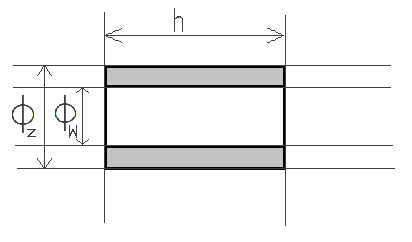
\includegraphics[width=11cm,height=6cm,angle=0]{schemat.png}'
%\label{fig:Schemat układu pomiarowego}
%\includegraphics[width=2cm,height=2cm,angle=90]{uwr.eps}
\end{figure} \\
- $\phi_w$ oznacza średnicę wewnętrzną \\
- $\phi_z$ oznacza średnicę zewnętrzną \\
-  $h$ oznacza wysokość (długość) tulejki

\subsection{Opis metody pomiarowej}
Tulejkę mierzymy według schematu - średnice wewnętrzną i zewnętrzną, dodatkowo długość tulejki, używając do tego śruby mikrometrycznej i suwmiarki. Pomiary wykonujemy kilkakrotnie, w różnych miejscach. Dodatkowo ważymy ciało kilkukrotnie, kładąc je w różnych miejscach na wadze.

\section{Wyniki pomiarów}
Wyniki pomiarów znajdują się w Tabeli 1, razem z niepewnościami (odczytanymi z urządzeń pomiarowych).
\begin{table}[]
    \centering
    \begin{tabular}{c|c|c|c|c|c|c|c|c|c}
        & $lp$ & $\phi_w$ & $\Delta_p \phi_w$ & $\phi_z$ & $\Delta_p \phi_z$ & $h$ & $\Delta_p h$ & $m$& $\Delta_p m$ \\ \hline
        & $1.$ &$11,85$	 &	$0,05$ &$16$ & $0,01$	& $22,05$	& $0,05$ & $5,17$ &$0,01$ \\
        & $2.$ & $12$ & $0,05$ & $16,01$ & $0,01$ & $22,5$ & $0,05$ & $5,41$ & $0,01$ \\
        & $3.$ & $12$ & $0,05$ & $16,01$ & $0,01$ & $22,45$ & $0,05$ & $5,7$ & $0,01$ \\
        & $4.$ & $11,75$ & $0,05$	& $16$ & $0,01$ & $22,4$ & $0,05$ & $5,49$ & $0,01 $\\
        & $5.$ & $11,8$ & $0,05$ & $16,01$ & $0,01$ & $22,5$ & $0,05$ & $5,64$ & $0,01$ \\
    \end{tabular}
    \caption{Wyniki pomiarów}
    \label{tab:my_label}
\end{table}

\subsection{Wzory}
Aby obliczyć wartość średnią pomiaru używamy wzoru:
\begin{equation*}
    \overline{\phi_w} = \frac{1}{n}\sum_{i=1}^n \phi_{wi}
\end{equation*}

Podobnie obliczamy pozostałe wartości średnie.

Na ich podstawie możemy obliczyć średnią objętość:
\begin{equation*}
    \overline{V} = \frac{\pi\overline{\phi_w}^2}{4}\overline{h} - \frac{\pi\overline{\phi_z}^2}{4}\overline{h}
\end{equation*}

\subsection{Przykładowe obliczenia + komentarze co jest liczone}

Aby obliczyć objętość, zaczniemy od wartości średnich wymiarów tulejki
\begin{equation*}
    \overline{\phi_w} = \frac{1}{5} \cdot (11,85 + 12 + 12 + 11,75 + 11,8) = 11,88
\end{equation*}
\begin{equation*}
    \overline{\phi_z} = \frac{1}{5} \cdot (16 + 16,01 + 16,01 + 16 + 16,01) = 16,006
\end{equation*}
\begin{equation*}
    \overline{h} = \frac{1}{5} \cdot (22,05 + 22,5 + 22,45 + 22,4 + 22,5) = 
     22,38
\end{equation*}

\subsection{Wyniki obliczeń}

Policzone według wspomnianych wzorów wartości średnie oraz niepewności przedstawiono w Tabeli 2.
\begin{table}[]
    \centering
    \begin{tabular}{c|c|c|c|c|c|c|c}
        $\overline{\phi_w}$ & $u(\overline{\phi_w})$ & $\overline{\phi_z}$ & $u(\overline{\phi_z})$ & $\overline{h}$ & $u(\overline{h})$ & $\overline{m}$ & $u(\overline{m})$ \\ \hline
        $11,88$ & $0,05902$ & $16,006$ & $0,00627163$ & $22,38$ & $0,0893495$ & $5,482$ & $0,0937408 $
    \end{tabular}
    \caption{Wartości średnie i niepewności}
    \label{tab:my_label}
\end{table}
Na podstawie tych wyników możemy obliczyć objętość średnią:
\begin{equation*}
    \overline{V} = \frac{\pi \cdot 11,88^2}{4} \cdot 22,38 - \frac{\pi \cdot 16,006^2}{4}\cdot 22,38 = 2022,392 [mm^3] = 2,022392 \cdot 10^{-6} [m^3]
\end{equation*}
Mając obliczoną średnią masę:
\begin{equation*}
    \overline{m} = \frac{1}{5} \cdot (5,17 + 5,41 + 5,7 + 5,49 + 5,64) = 
     5,482 [g] = 5,482 \cdot 10^{-3} kg
\end{equation*}
możemy obliczyć średnią gęstość tulejki:
\begin{equation*}
    \overline{\rho} = \frac{\overline{m}}{\overline{V}} = \frac{5,482 \cdot 10^{-3} kg}{2,022392 \cdot 10^{-6}[m^3]} = 2,710651 \cdot 10^3 \frac{kg}{m^3}
\end{equation*}

\subsection{Analiza niepewności pomiarowych}
Biorąc pod uwagę różnicę poszczególnych pomiarów i wartości średniej należy obliczyć niepewnoś (typu A)
    $$u_A(\overline{x}) = \sqrt{\frac{1}{n(n-1)}\sum_{i=1}^n (x_i-\overline{x})^2} $$
Urządzenia pomiarowe dają wyniki obarczone błędem, co należy uwzględnić w obliczeniach (niepewność typu B)
    $$u_B(x) = \sqrt{\frac{(\Delta_px)^2}{3} + \frac{(\Delta_ex)^2}{3} + \frac{(\Delta_tx)^2}{3} } $$
Końcowa niepewność pomiaru danej wielkości:
    $$u(\overline{x}) = \sqrt{u_A^2 + u_B^2 }$$
Dodatkowo, jeśli dana wielkość jest zależna od innych, jej niepewność nazywamy niepewnością złożoną i obliczamy ze wzoru:
\begin{equation*}
    u_c(y) = \sqrt{\sum_{i=1}^k \left( \frac{\partial y}{\partial x_i} u(x_i)\right)^2}
\end{equation*}

Korzystamy z podanych wzorów i uzyskujemy niepewność średnicy wewnętrzej typu A:
\begin{equation*}
   u_A(\overline{\phi_w}) = \sqrt{\frac{1}{5(5-1)}\sum_{i=1}^5 (\phi_{wi}-\overline{\phi_w})^2}
\end{equation*}
\begin{equation*}
   = \sqrt{\frac{1}{20} ((11,85-11,88)^2 + (12-11,88)^2 + (12-11,88)^2 + (11,75-11,88)^2 + (11,8-11,88)^2)} 
\end{equation*}
\begin{equation*}
    = 0,0514781507 [mm]
\end{equation*}
tupu B:
\begin{equation*}
    u_B(\phi_w) = \sqrt{\frac{(\Delta_p\phi_W)^2}{3}} 
    = \sqrt{\frac{(0,05)^2}{3}} = 0,02886751346 \ [mm]
\end{equation*}
oraz niepewność ogólną (z oczywistych względów nie uwzględniamy niepewości czasu, oceniamy również wzrok eksperymentatora na wystarczająco dobry): 

\begin{equation*}
    u(\overline{\phi_w}) = \sqrt{u_A^2(\overline{\phi_w}) + u_B^2(\phi_w) }
    = \sqrt{ 0,0514781507^2+ 0,02886751346^2 } 
\end{equation*}
\begin{equation*}= 0,0590197707\ [mm]
\end{equation*}
Podobnie obliczamy pozostałe niepewności oraz niepewność złożoną objętości:
\begin{equation*}
    u_c(V) = \sqrt{\left( \frac{\partial \overline{V}}{\partial \overline{\phi_z}} u(\overline{\phi_z})\right)^2 + \left(\frac{\partial \overline{V}}{\partial \overline{\phi_w}} u(\overline{\phi_w}) \right)^2 + \left(\frac{\partial \overline{V}}{\partial \overline{h}} u(\overline{h}) \right)^2} 
\end{equation*}
\begin{equation*}
    = \sqrt{\left( \frac{\pi\overline{\phi_z}}{2} u(\overline{\phi_z})\right)^2 + \left(\frac{\pi\overline{\phi_w}}{2} u(\overline{\phi_w})\right)^2 + \left(\frac{\pi}{4}(\overline{\phi_w}^2 - \overline{\phi_z}^2) u(\overline{h})\right)^2}
\end{equation*}
co po podstawieniu wartości daje wynik:
\begin{equation*}
    u_c(\overline{V}) = 26,17639344 \ [mm^3]
\end{equation*}
Do wyniku potrzebujemy ostateczną niepewność $u_c(\rho)$, którą obliczymy z tego samego wzoru:
\begin{equation*}
    u_c(\overline{\rho}) = \sqrt{\left( \frac{\partial \overline{\rho}}{\partial \overline{V}} u(\overline{V}) \right)^2 + \left( \frac{\partial \overline{\rho}}{\partial \overline{m}} u(\overline{m}) \right)^2 } 
    = \sqrt{\left( \frac{-\overline{m}}{\overline{V}^2} u(\overline{V}) \right)^2 + \left( \frac{1}{\overline{V}} u(\overline{m}) \right)^2 }
\end{equation*}
\begin{equation*}
    = 0,00005813254425
\end{equation*}
\subsection{Wyniki końcowe}
Obliczona niepewność wyniku to $0,00005813254425$, po zaokrągleniu do dwóch cyfr znaczących otrzymujemy $5,9 \cdot 10^{-5} \frac{g}{mm^3}$, co można zamienić na 
$5,9 \cdot 10 \frac{kg}{m^3}$.
Zaokrąglimy teraz wynik do tego samego rzędu wielkości 
$$2,710651099 \cdot 10^3 \frac{kg}{m^3} \approx 2711 \frac{kg}{m^3} $$

Ostateczny wynik naszego eksperymentu zapisujemy jako 
$$ \overline{\rho} = (2,711 \pm 0,059) \cdot 10 ^3 \frac{kg}{m^3} $$
\section{Wnioski}
Udało nam się obliczyć gęstość metalowej tulejki na podstawie jej masy oraz wymiarów. Wzięliśmy pod uwagę niepewności urządzeń pomiarowych; suwmiarki, śruby mikrometrycznej i wagi, oraz obliczone niepewności wynikające z odchylenia poszczególnych pomiarów od wartości średniej. Porównując wynik ze znanymi gęstościami metali można wnioskować, że badana tulejka została wykonana z aluminium.

\end{document}
